\documentclass[10pt]{article}
\usepackage{float}
\RequirePackage{eso-pic}
\usepackage{caption}
\captionsetup[table]{labelformat=empty}



\usepackage{geometry}
\geometry{
a4paper,
left=11mm,
right=14mm,
top=37mm,
bottom=14mm,
}



\usepackage{colortbl}
\usepackage{fontspec}
\setmainfont[Ligatures=TeX]{Calibri}



\newcommand\BackgroundPic{%
\put(0,0){%
\parbox[b][\paperheight]{\paperwidth}{%
\vfill
\centering
\includegraphics{MBIE_generic_background.pdf}%
\vfill
}}}



\begin{document}
\thispagestyle{empty}
\AddToShipoutPicture{\BackgroundPic}
\section*{Key Export Statistics\footnotemark - Chocolate\footnotemark }
\today\\
\begin{table}[ht]
\centering
{\scriptsize
\begin{tabular}[t]{p{1.8cm}>{\hfill}p{1.4cm}>{\hfill}p{1.4cm}>{\hfill}p{1.6cm}>{\hfill}p{1.9cm}>{\hfill}p{2cm}>{\hfill}p{1.9cm}>{\hfill}p{1.5cm}}
 \textbf{Country} & \textbf{Yearly Qty} & \textbf{Yearly Value} & \textbf{Yearly Price} & \textbf{3Year CAGR(Qty)} & \textbf{3Year CAGR(Value)} & \textbf{3Year CAGR(Price)} & \textbf{Price Elasticity} \\
\hline
Australia & 9,197 & 86.6 & \$9.4 & 4.9\% & 6.7\% & 1.7\% & 3.0 \\  
China & 237 & 3.4 & \$14.1 & 107.6\% & 117.3\% & 4.7\% & 22.9 \\  
Malaysia & 227 & 3.0 & \$13.3 & 13.9\% & 23.8\% & 8.6\% & 1.6 \\  
U.A.E & 58 & 1.1 & \$19.2 & 346.8\% & 234.7\% & -25.1\% & -13.8 \\  
Hong Kong & 54 & 0.9 & \$16.8 & 32\% & 43.7\% & 8.9\% & 3.6 \\  
South Korea & 65 & 0.9 & \$13.9 & 11.5\% & 16.4\% & 4.5\% & 2.6 \\  
Other & 513 & 6.4 & \$12.5 & 1\% & 5.6\% & 4.6\% & 0.2 \\  
Total & 10,350 & 102.3 & \$9.9 & 5.9\% & 8.7\% & 2.6\% & 2.2 \\  
\hline
\end{tabular}
}
\caption{\scriptsize Top 6 Chocolate Markets for year ending November - 2015: Quantity('000 kg) Value(NZ\$Mill), Price and their last 3-Year Growth Rates}
\end{table}


\vspace{-0.7cm}



   \begin{figure}[H]
   \centering
    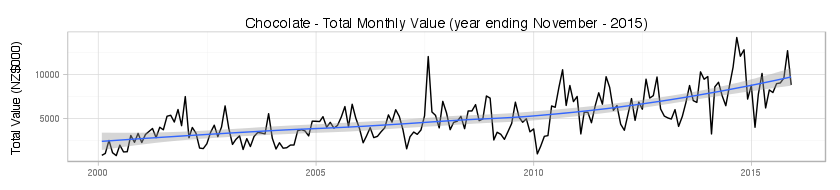
\includegraphics[scale=0.5]{../graphs/monthly_value/chocolate_monthly_value.png} \
    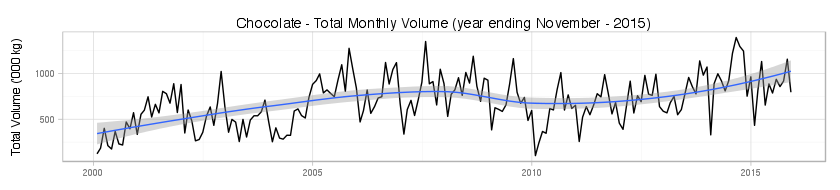
\includegraphics[scale=0.5]{../graphs/monthly_volume/chocolate_monthly_volume.png} \
    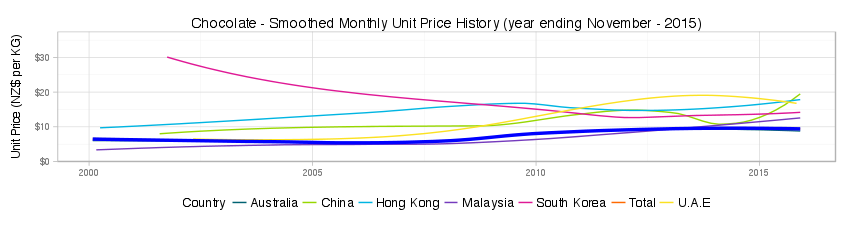
\includegraphics[scale=0.5]{../graphs/smoothed_price/chocolate_smoothed_price.png} \
    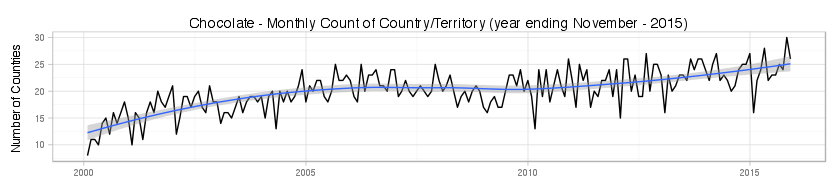
\includegraphics[scale=0.5]{../graphs/monthly_number_countries/chocolate_monthly_count.png} \
    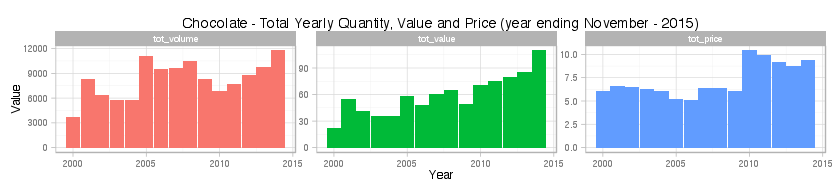
\includegraphics[scale=0.5]{../graphs/yearly_summary/chocolate_yearly_summary.png} \
   \end{figure}



\footnotetext[1]{Source: Statistics New Zealand - Overseas Merchandise Trade}
\footnotetext[2]{Harmonised System Codes for Chocolate starting with: 180631, 180632, 180690.}
\end{document}
